% gradient-descent.tex — \input'd from thesis/experiments.tex
%
% Large-scale gradient ascent on sys for F=10 polytopes.
%
% Sources:
%   - Generated data: experiments/gradient-descent/gradient-descent.jsonl
%   - Plot script: experiments/gradient-descent/gradient_descent.py
%   - Developer notes: experiments/gradient-descent/README.md
%   - Builds on: sec:sys-optimization (method, derivative formulae)
%   - Prose: agent-written, unreviewed
%
% Structure:
%   - Motivation (scaling up sys-optimization)
%   - Experimental setup (two polytope classes, backends)
%   - Results (distribution, by-class breakdown)
%   - Discussion (comparison with sys-optimization, interpretation)

\subsection{Large-Scale Gradient Ascent on sys}
\label{sec:gradient-descent}

Section~\ref{sec:sys-optimization} developed the gradient
$\nabla_{(h,n)}\,\mathrm{sys}$ and demonstrated iterative gradient ascent
on 140~polytopes with $F \le 10$, reaching a maximum
$\mathrm{sys} \approx 0.88$.
This section scales the procedure to ${\sim}1000$ starting polytopes,
all with $F = 10$, and distinguishes two structural classes:
general polytopes and Lagrangian products.

\subsubsection*{Setup}

We generate two classes of random $F = 10$ polytopes:
\begin{enumerate}
\item \emph{General polytopes} ($N = 500$):
  normals uniform on~$S^3$, heights uniform in~$[0.8, 1.2]$.
  Uses the pruned HK2017 algorithm
  (Corollary~\ref{cor:adjacency-pruning}).

\item \emph{Lagrangian products} ($N = 501$, three buckets of~$167$):
  random polygon pairs $K_q \times_L K_p$ with facet splits
  $(F_q, F_p) \in \{(3,7),\,(4,6),\,(5,5)\}$.
  Gradient ascent uses the billiard algorithm
  (Theorem~\ref{thm:billiard-characterization}) with directed
  $\omega_0$~pruning.
  Normal perturbations are projected to preserve the Lagrangian product
  structure: $q$-facet normals remain in the $q$-plane, $p$-facet normals
  remain in the $p$-plane.
\end{enumerate}

The gradient computation and step bound follow
Section~\ref{sec:sys-optimization} exactly:
derivatives via the envelope theorem
(Lemmas~\ref{lem:vol-derivative}--\ref{lem:cap-derivative-normal},
Corollary~\ref{cor:sys-derivative}),
step bound preserving the combinatorial type,
line search over step fractions
$\{0.1,\, 0.25,\, 0.5,\, 0.75,\, 0.95\} \cdot t_{\max}$
comparing height-only and $(h,n)$ directions.
Iteration terminates when the best step improves $\mathrm{sys}$
by less than~$10^{-6}$, or after 20~iterations.

\subsubsection*{Results}

Of the 1001 starting polytopes, 995 produce at least one valid gradient
step (6~fail due to degenerate initial capacity or volume).

\begin{figure}[ht]
\centering
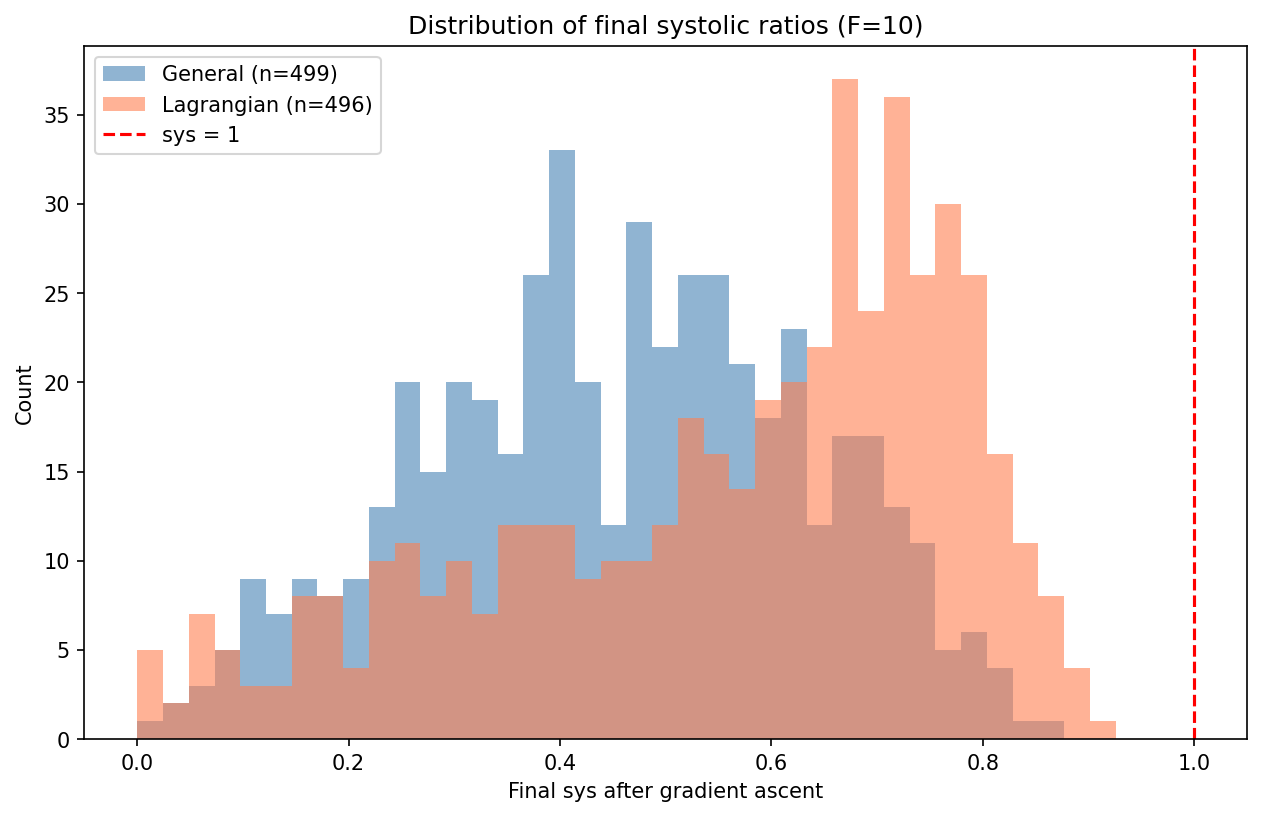
\includegraphics[width=\textwidth]{../experiments/gradient-descent/gradient_descent_results.png}
\caption{Distribution of final $\mathrm{sys}$ after gradient ascent
  for $F = 10$ polytopes.
  Lagrangian products (coral) cluster at higher values than general
  polytopes (blue).
  No polytope reaches $\mathrm{sys} = 1$ (dashed line).}
\label{fig:gd-histogram}
\end{figure}

\begin{figure}[ht]
\centering
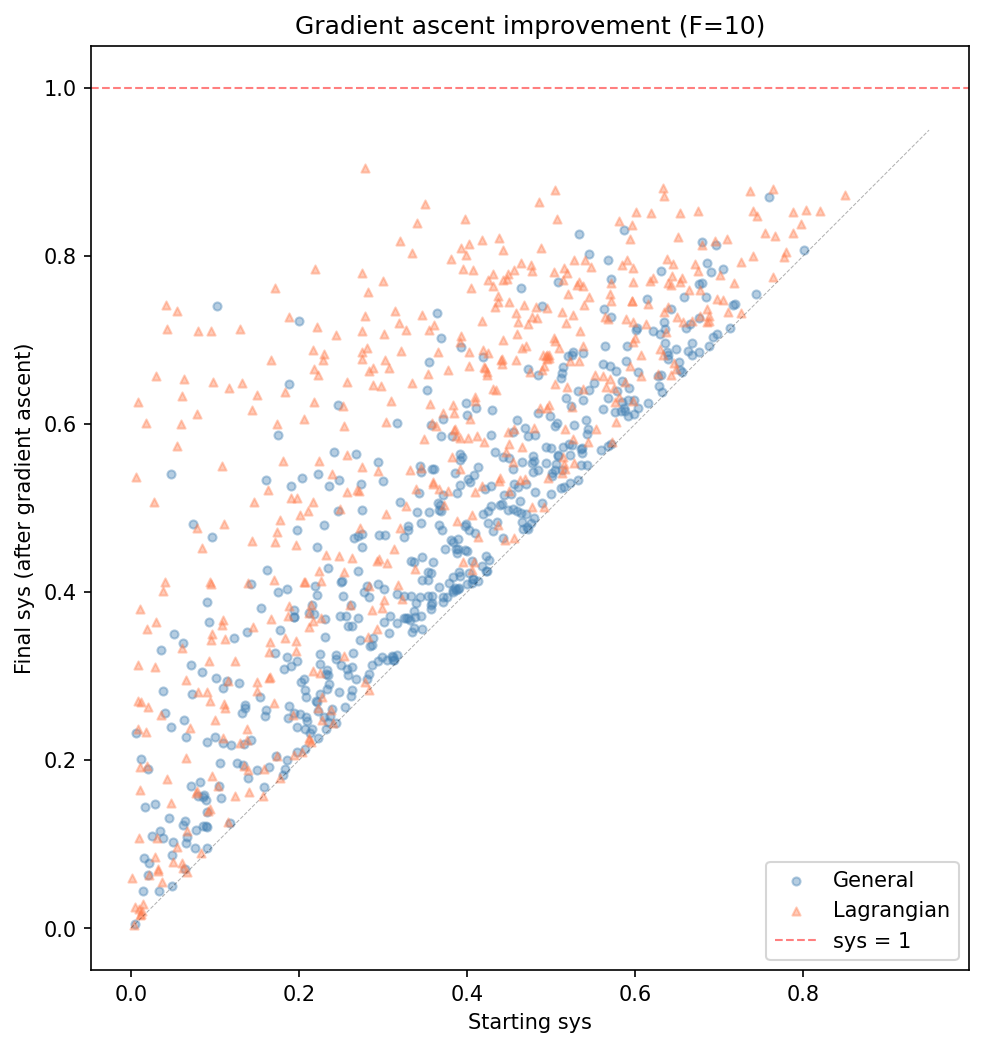
\includegraphics[width=\textwidth]{../experiments/gradient-descent/gradient_descent_scatter.png}
\caption{Starting vs.\ final $\mathrm{sys}$ under gradient ascent.
  Nearly all points lie above the diagonal, confirming that the
  gradient procedure reliably improves $\mathrm{sys}$.
  The improvement is largest for polytopes starting at low
  $\mathrm{sys}$; high-starting polytopes have less room to improve.}
\label{fig:gd-scatter}
\end{figure}

\begin{table}[ht]
\centering
\begin{tabular}{lrrrrr}
\toprule
Type & $N$ & Mean sys & Max sys & P90 sys & Mean $\Delta$ \\
\midrule
General       & 499 & 0.453 & 0.870 & 0.687 & 0.100 \\
Lagrangian 3$\times$7 & 166 & 0.493 & 0.862 & 0.781 & 0.182 \\
Lagrangian 4$\times$6 & 166 & 0.566 & 0.881 & 0.784 & 0.222 \\
Lagrangian 5$\times$5 & 164 & 0.628 & 0.905 & 0.806 & 0.217 \\
\bottomrule
\end{tabular}
\caption{Summary statistics by polytope class.
  $\Delta$ is the improvement from starting to final $\mathrm{sys}$.}
\label{tab:gd-summary}
\end{table}

\textbf{No polytope achieves $\mathrm{sys} > 1$.}
The overall maximum is $\mathrm{sys} \approx 0.905$,
attained by a $5 \times 5$ Lagrangian product.
Only one polytope exceeds $\mathrm{sys} = 0.9$.

Three patterns emerge from the class comparison
(Table~\ref{tab:gd-summary}, Figures~\ref{fig:gd-histogram}
and~\ref{fig:gd-scatter}):
\begin{enumerate}
\item \emph{Lagrangian products reach higher $\mathrm{sys}$ than general
  polytopes} (mean~$0.56$ vs.~$0.45$, max~$0.905$ vs.~$0.870$),
  consistent with the known counterexample being a Lagrangian product.

\item \emph{More balanced splits achieve higher $\mathrm{sys}$}:
  the $5 \times 5$ split (mean~$0.628$) outperforms $4 \times 6$
  ($0.566$) and $3 \times 7$ ($0.493$).
  The counterexample of Haim-Kislev and Ostrover~\cite{HaimKislevOstrover2024}
  is a $5 \times 5$ product, consistent with this trend.

\item \emph{Gradient ascent substantially improves $\mathrm{sys}$}:
  mean improvement $+0.10$ for general polytopes
  and $+0.18$--$0.22$ for Lagrangian products.
  After optimization, 69\% of polytopes converge
  (improvement $< 10^{-6}$) within 20~iterations.
\end{enumerate}

\subsubsection*{Discussion}

Compared to Section~\ref{sec:sys-optimization}, this experiment
uses~$7\times$ more starting polytopes and distinguishes Lagrangian
products from general polytopes, but the qualitative conclusion is
the same: gradient ascent does not push $\mathrm{sys}$ past~$1$.
The maximum increases slightly ($0.905$ vs.~$0.878$), but remains
well below the Viterbo threshold.

\subsubsection*{Distribution shift}

Figure~\ref{fig:gd-density} overlays kernel density estimates
of the starting and final $\mathrm{sys}$ distributions
for both polytope classes.
Gradient ascent shifts the Lagrangian distribution rightward
into a concentrated peak near $\mathrm{sys} \approx 0.7$,
while the general distribution shifts more modestly
and remains spread across $[0.2, 0.85]$.
Both final distributions drop sharply to zero
well below $\mathrm{sys} = 1$, with no density near the
Viterbo threshold.

\begin{figure}[ht]
\centering
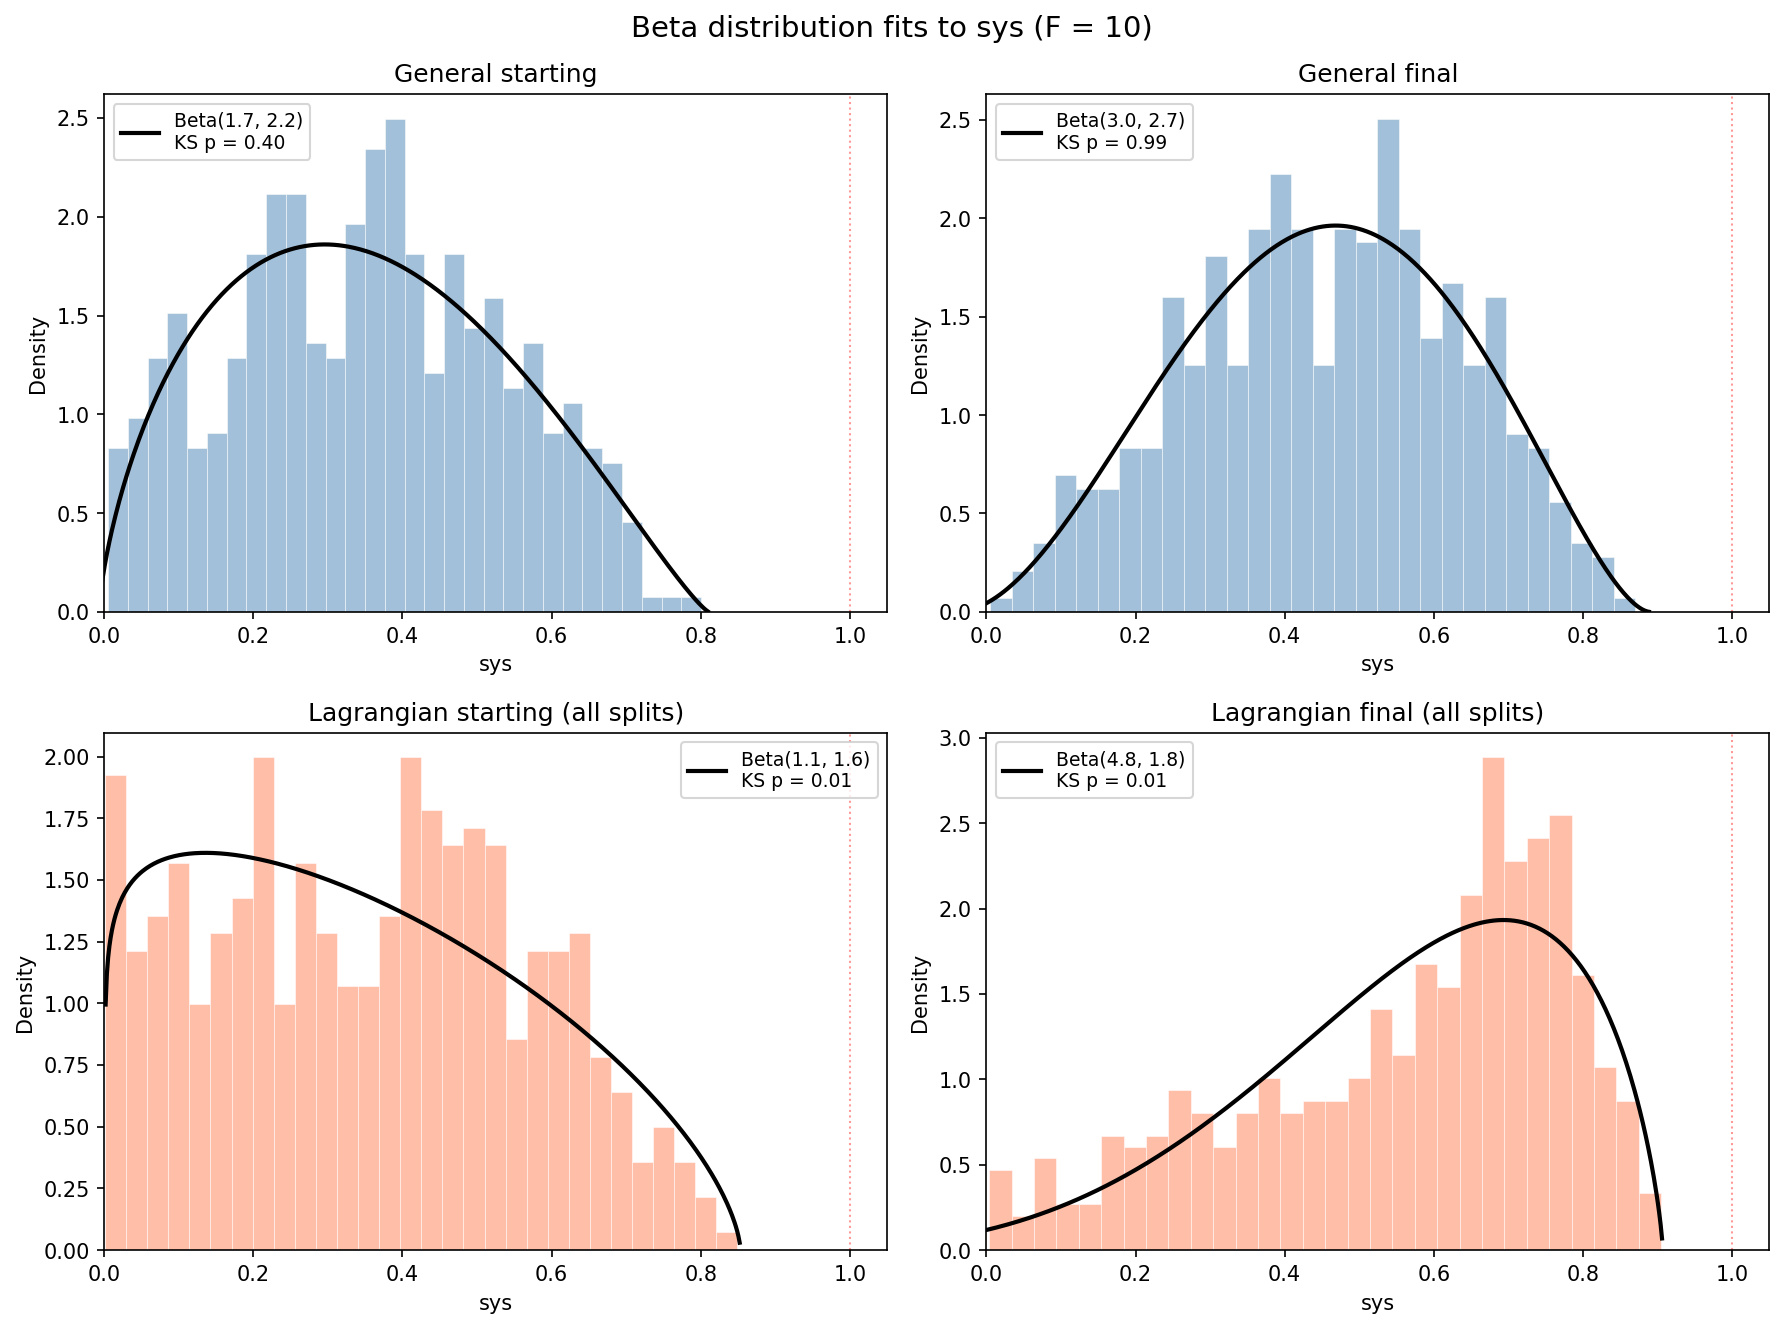
\includegraphics[width=\textwidth]{../experiments/gradient-descent/gradient_descent_density.png}
\caption{Kernel density estimates of $\mathrm{sys}$ before (dashed)
  and after (solid) gradient ascent.
  Optimization concentrates the Lagrangian distribution around
  $\mathrm{sys} \approx 0.7$;
  the general distribution shifts modestly rightward.
  Both vanish before $\mathrm{sys} = 1$.}
\label{fig:gd-density}
\end{figure}

\subsubsection*{Convergence quality}

The gradient norms at termination reveal that the algorithm does
\emph{not} find approximate local maxima.
The median height gradient $\|\nabla_h\,\mathrm{sys}\|$ at termination
is~$0.36$ for general polytopes and~$0.53$ for Lagrangian products;
the median normal gradient $\|\nabla_n\,\mathrm{sys}\|$ is~$1.4$
and~$1.2$, respectively (Figure~\ref{fig:gd-convergence}).
These are $O(1)$ values---far from the near-zero gradients
expected at a local maximum.

\begin{figure}[ht]
\centering
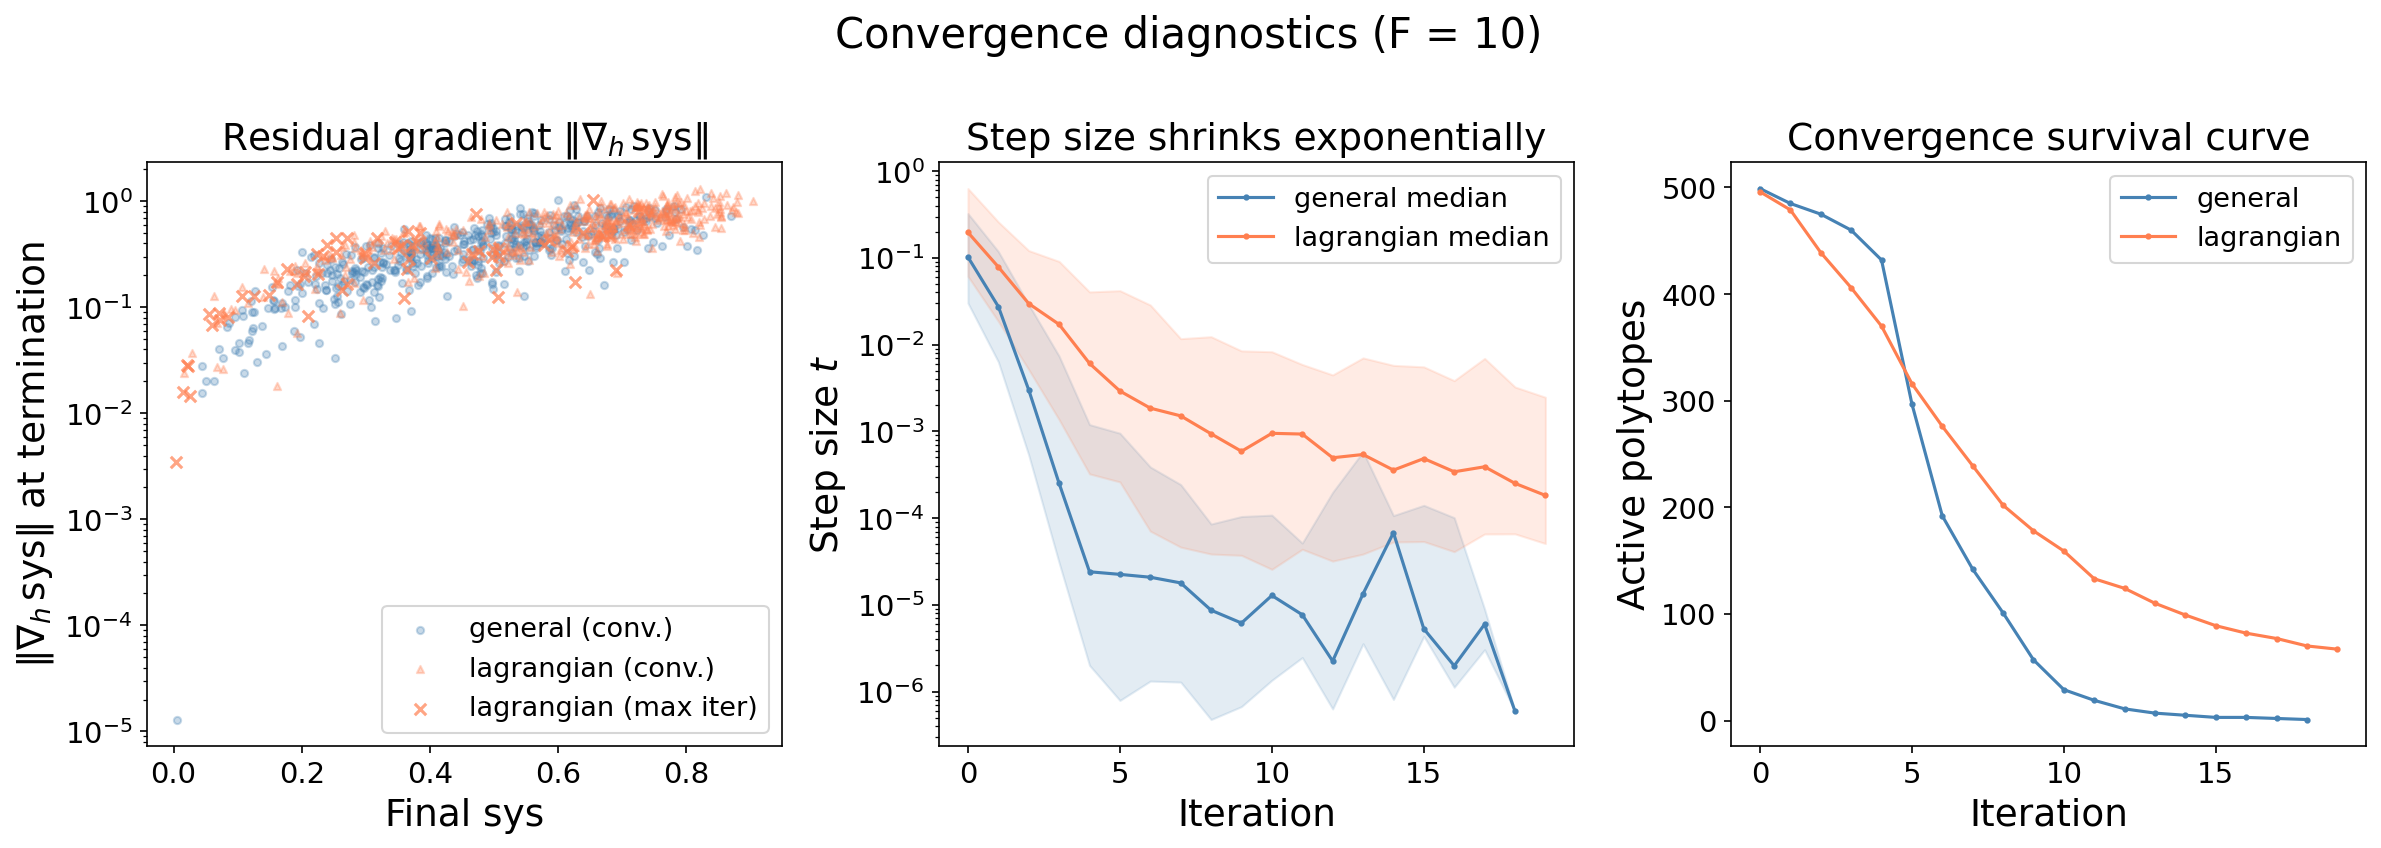
\includegraphics[width=\textwidth]{../experiments/gradient-descent/gradient_descent_convergence.png}
\caption{Gradient norms at termination vs.\ final $\mathrm{sys}$.
  Left: height gradient $\|\nabla_h\,\mathrm{sys}\|$
  shows a positive correlation ($r \approx 0.80$)---polytopes
  with higher $\mathrm{sys}$ have \emph{larger} residual gradients.
  Right: normal gradient $\|\nabla_n\,\mathrm{sys}\|$ is uncorrelated.
  Crosses mark polytopes that exhausted 20~iterations
  (67~Lagrangian products, 0~general).}
\label{fig:gd-convergence}
\end{figure}

The algorithm converges because the step bound~$t_{\max}$
shrinks, not because the gradient vanishes.
Figure~\ref{fig:gd-stepsize} shows the dynamics:
the median step size~$t_{\mathrm{actual}}$ drops exponentially
from~${\sim}0.1$ at iteration~$0$ to~${\sim}10^{-4}$ by iteration~$10$.
Meanwhile, the line search consistently selects the most aggressive
fraction ($0.95 \cdot t_{\max}$) in 87\% of all iterations.
This means the algorithm always wants to step as far as possible,
but the combinatorial type boundary closes in,
leaving less and less room for improvement.

\begin{figure}[ht]
\centering
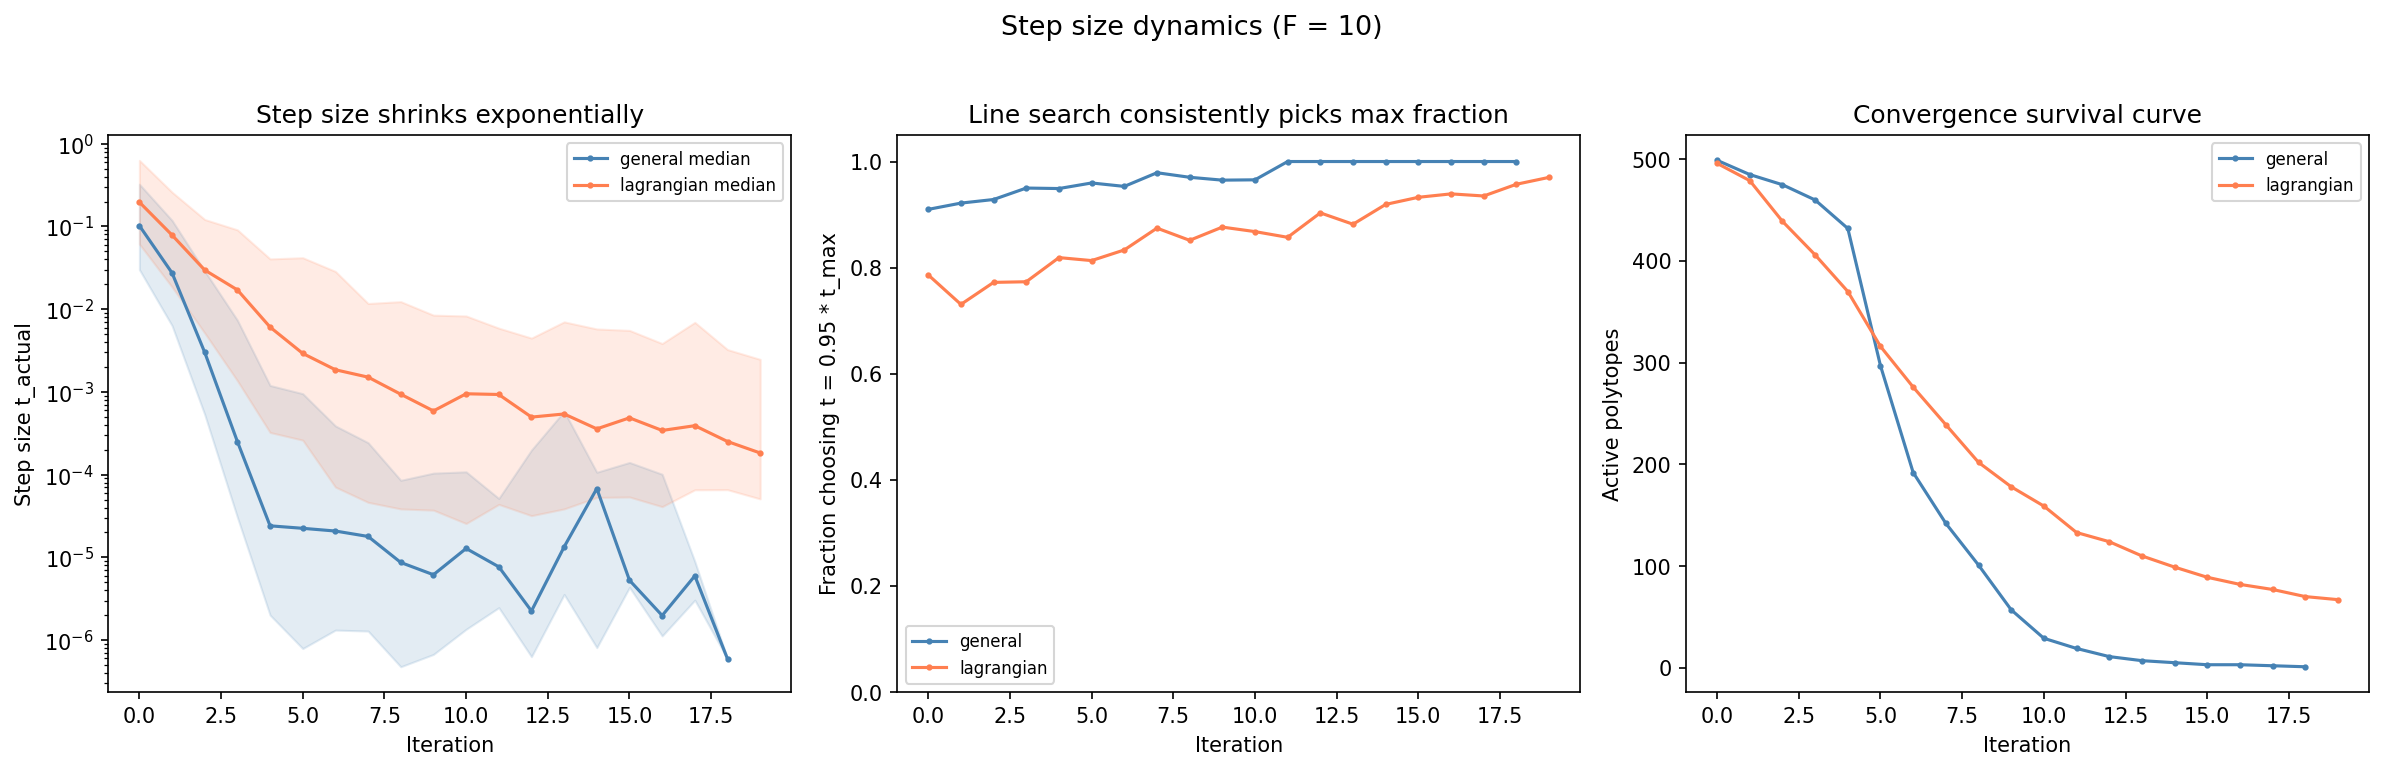
\includegraphics[width=\textwidth]{../experiments/gradient-descent/gradient_descent_stepsize.png}
\caption{Step size dynamics.
  Left: median step size (with IQR shading) shrinks
  exponentially as the polytope approaches its combinatorial
  type boundary.
  Center: the line search picks $0.95 \cdot t_{\max}$
  in ${\sim}85$--$95\%$ of iterations.
  Right: survival curve showing how many polytopes remain
  active (have not yet converged) at each iteration.}
\label{fig:gd-stepsize}
\end{figure}

The positive correlation between final $\mathrm{sys}$ and
$\|\nabla_h\,\mathrm{sys}\|$ ($r \approx 0.80$;
Figure~\ref{fig:gd-convergence}, left) is notable:
the polytopes closest to the Viterbo threshold have the
\emph{strongest} upward gradients, yet are the most
constrained by the step bound.
This suggests that the $\mathrm{sys} < 1$ barrier
is not a gradient obstruction but a \emph{step-bound barrier}---the
combinatorial type cell does not extend far enough in the
direction of increasing $\mathrm{sys}$.

\subsubsection*{Interpretation}

The clear gap between the observed maximum (${\approx}0.905$) and the
threshold~$1$ thus reflects a limitation of the optimization
method, not necessarily the absence of counterexamples at $F = 10$.
Three factors contribute:
\begin{itemize}
\item The combinatorial-type-preserving step bound confines each step
  to the current polytope's cell in parameter space.
  Crossing into a new cell requires restarting---our
  greedy line search does not do this.
\item The basin of attraction for $\mathrm{sys} > 1$ (if it exists at
  $F = 10$) may have small measure, so random starting points are
  unlikely to land in it.
\item The counterexample of~\cite{HaimKislevOstrover2024} uses a regular
  pentagon with specific geometric structure that random
  polygon pairs do not approximate.
\end{itemize}
